\documentclass[12pt,twosides,onecolumn,openany]{article}
\usepackage{graphicx} 


\usepackage[catalan]{babel}
\usepackage{emptypage}
\usepackage{hyperref}
\usepackage{mathtools}
\usepackage{blindtext}
\usepackage{subfigure}
\usepackage[utf8]{inputenc}
\usepackage{caption}
\usepackage{subcaption}
\usepackage{wrapfig}
\usepackage[a4paper]{geometry}
\geometry{top=2.5cm, bottom=2.5cm, left=2.5cm, right=2.5cm}
\usepackage{fancyhdr}
\pagestyle{fancy}
\usepackage{amsmath}
\usepackage{amssymb}
\usepackage{amsfonts}
\providecommand{\norm}[1]{\lVert#1\rVert}
\hypersetup{colorlinks=true,urlcolor=blue,linkcolor=blue}
\usepackage{multirow}
\usepackage{multicol}
\usepackage{rotating}

\usepackage{titlesec}

\newenvironment{Figura}
  {\par\medskip\noindent\minipage{\linewidth}}
  {\endminipage\par\medskip}

\titleformat{\section}  % comando de sección a formatear
  {\fontsize{14}{16}\bfseries} % formato para toda la línea
  {\thesection} % cómo mostrar el número
  {0.4em} % espacio entre el número y el texto
  {} % formato solo para el texto
  [] % formato para después del texto


\fancyhf{}
\fancyhead[LO,RE]{Grup D3}
\fancyhead[RO,LE]{Pràctica Ia}
\fancyfoot[LO,RE]{\thepage}
\fancyfoot[RO,LE]{Laboratori de Termodinàmica - UAB}
\graphicspath{ {images/} }

\begin{document}

\begin{center}
    {\Large \textsc{Transport de la calor: Estudi del transport de la calor en una barra metàl·lica}}\\
    \vspace{0.2cm}
    \textsc{30 d'Octubre de 2024}\\
    \vspace{0.2cm}
    $\begin{matrix} 
    \text{Miguel A.} \hspace{1.5cm} & \text{Daniel B.} & \hspace{1.5cm} \text{Sergi R.}\\1637738 \hspace{1.5cm} & 1603508 & \hspace{1.5cm} 1607805
    \end{matrix}$
\end{center}
\begin{center}
    \textsc{\textit{RESUM}}
\end{center}
Lorem ipsum dolor sit amet, consectetur adipiscing elit, sed do eiusmod tempor incididunt ut labore et dolore magna aliqua. Ut enim ad minim veniam, quis nostrud exercitation ullamco laboris nisi ut aliquip ex ea commodo consequat. Duis aute irure dolor in reprehenderit in voluptate velit esse cillum dolore eu fugiat nulla pariatur. Excepteur sint occaecat cupidatat non proident, sunt in culpa qui officia deserunt mollit anim id est laborum. \cite{prueba}
\vspace{0.5cm}
\begin{multicols}{2}
\section{Introducció i objectius}
\begin{equation}\label{sol_estacionaria}
  \theta(x) = \theta_0e^{-px}
\end{equation}
\begin{multline}\label{sol_permanent}
  \theta(x,t) = \theta_0e^{-px} +\\
   + A_0e^{-mx}\cos{\left( \frac{2\pi}{\tau} -hx \right)} 
\end{multline}
\begin{equation}\label{prom_temp}
  \langle \theta(x,t) \rangle = \theta_0e^{-px}  
\end{equation}
\section{Resultats i discussió}
\subsection{Estat estacionari}
Segons el desenvolupament teòric que seguim no podem negligir les diferències de radi entre les tres barres metàl·liques. Mesurem a l'inici, al mig i al final el diàmetre de cada barra i obtenim els valors de la Taula \ref{Tau:diam_radis}.
\begin{Figura}
  \centering
  \captionof{table}{\footnotesize{Diametres i radis de cada metall}}
  \begin{tabular}{c|c|c}
    a & a & a\\
    \hline\hline
    b & b & b
  \end{tabular}
  \label{Tau:diam_radis}
\end{Figura}
A més, al llarg de l'experiment el labortaori ha anat canviant lleugerament de temperatura ambient. Per aquest motiu a l'hora de calcular els increments de temperatura $\theta_x$ farem servir com a temperatura ambient de referència la mitjana de tres mesures (veure Taula \ref{T_ambient} a l'Annex). Per tant, el valor de la temperatura ambient al laboratori és: \(T_a = ( \pm )\,\text{K}\).\\\\
A partir de les dades de temperatura obtingudes per a cada barra obtenim la gràfica de la Figura \ref{DeltaT_vs_d}. Es pot veure com l'increment de temperatura decau de forma exponencial amb la distància al punt calent, tal com es podia preveure del desenvolupament teòric (equació \eqref{sol_estacionaria}). Fent servir codi en Python obtenim un ajust exponencial de les dades mesurades. Aquest ajust es pot observar també a la figura \ref{DeltaT_vs_d}, i les dades dels coeficients ajustats a la Taula \ref{Tau:coef_exponencial}
\begin{Figura}
  \centering
  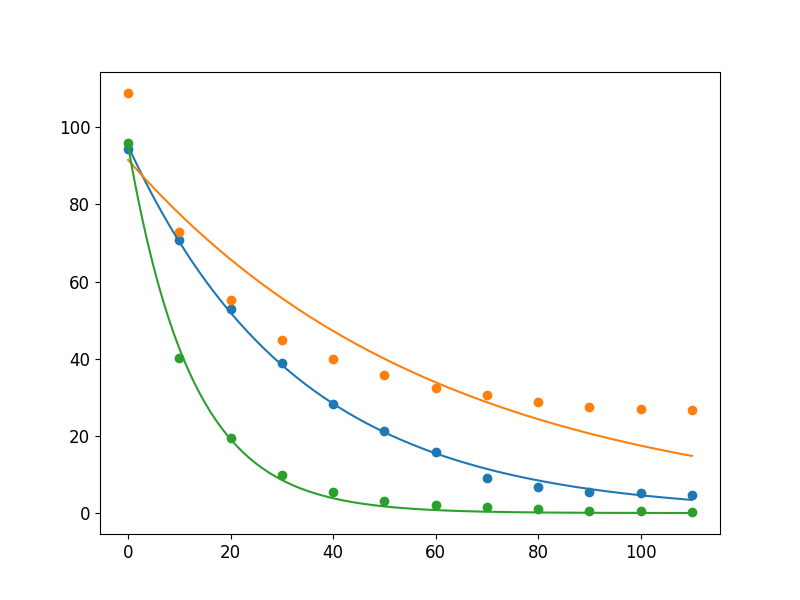
\includegraphics[width = 1\linewidth]{../../graphs/practica_Ia/plots/ln_theta.png}\label{DeltaT_vs_d}
  \captionof{figure}{\footnotesize{Prova}}
\end{Figura}

\begin{Figura}
  \centering
  \captionof{table}{\footnotesize{Coeficients $a$ i $b$ de l'ajust exponencial $y = ae^{bx}$ per als punts experimentals mesurats per l'alumini, el llautó i el ferro.}}
  \begin{tabular}{c|c|c}
    a & a & a\\
    \hline
    b & b & b
  \end{tabular}
  \label{Tau:coef_exponencial}
\end{Figura}
Per a trobar el valor experimental de $p$ apliquem logaritme als valors experimentals per a poder realitzar una regressió lineal. Observem aquestes dades experimentals i les rectes de regressió a la Figura \ref{lnDeltaT_vs_d}. A la Taula \ref{Tau:dades_regressio} queden
\begin{Figura}
  \centering
  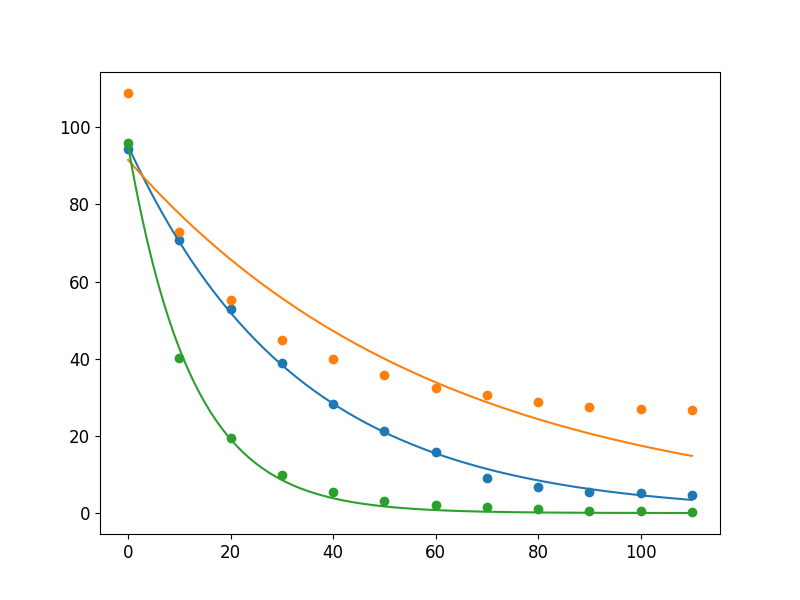
\includegraphics[width = 1\linewidth]{../../graphs/practica_Ia/plots/ln_theta.png}\label{lnDeltaT_vs_d}
  \captionof{figure}{\footnotesize{Prova}}
\end{Figura}           

\begin{Figura}
  \centering
  \captionof{table}{\footnotesize{Dades regresió.}}
  \begin{tabular}{c|c|c}
    a & a & a\\
    \hline\hline
    b & b & b
  \end{tabular}
  \label{Tau:dades_regressio}
\end{Figura}
Tenint en compte de l'equació \eqref{sol_estacionaria} què val $p$ i suposant el mateix valor constant del coeficient $\lambda$ per als tres metalls observem la temperatura d'un metall decau com $(Kr)^{1/2}$. Deduim doncs que la conductivitat tèrmica dels tres metalls és diferent 
\begin{equation*}
  K_a < K_b < K_c \hspace{3mm}
\end{equation*}
i que existeixen les relacions
\begin{equation*}
  \frac{K_ir_i}{K_jr_j} = \frac{p^2_j}{p^2_i}
\end{equation*}
on $i$ i $j$ prenen valors dels diferents metalls que estem estudiant. Fent recerca a la literatura trobem el valor de la conductivitat tèrmica del ferro: \(K_{\text{Fe}} = (\pm) \, \text{V}/\text{mK}\). Fent servir les relacions anteriors i el valor trobat a la literatura podem calcular, aproximadament, els valors de la conductivitat tèrmica dels altres dos metalls. Podem comparar aquests valors obtinguts amb els que podem trobar a la literatura. S'observen totes aquestes dades a la Taula \ref{Tau:conductivitats_termiques_Fe}
\begin{Figura}
  \centering
  \captionof{table}{\footnotesize{Comparació conductivitats tèrmiques - Patró ferro}}
  \begin{tabular}{c|c|c}
    a & a & a\\
    \hline\hline
    b & b & b
  \end{tabular}
  \label{Tau:conductivitats_termiques_Fe}
\end{Figura}
Com a aproximació alternativa podem fer servir, en comptes del ferro, l'alumini com a patró. Aplicant les mateixes relacions que amb el ferro obtenim les dades de la Taula \ref{Tau:conductivitats_termiques_Al}
\begin{Figura}
  \centering
  \captionof{table}{\footnotesize{Comparació conductivitats tèrmiques - Patró alumini}}
  \begin{tabular}{c|c|c}
    a & a & a\\
    \hline\hline
    b & b & b
  \end{tabular}
  \label{Tau:conductivitats_termiques_Al}
\end{Figura}
\textit{Explicaciones varias}
\subsection{Estat permanent}
A partir de les dades obtingudes experimentalment representem l'evolució temporal de la temperatura segons cada posició de la barra gran, Figura \ref{fig:T_vs_t_gran}, i de la barra petita, \ref{fig:T_vs_t_petita}.
\begin{Figura}
  \centering
  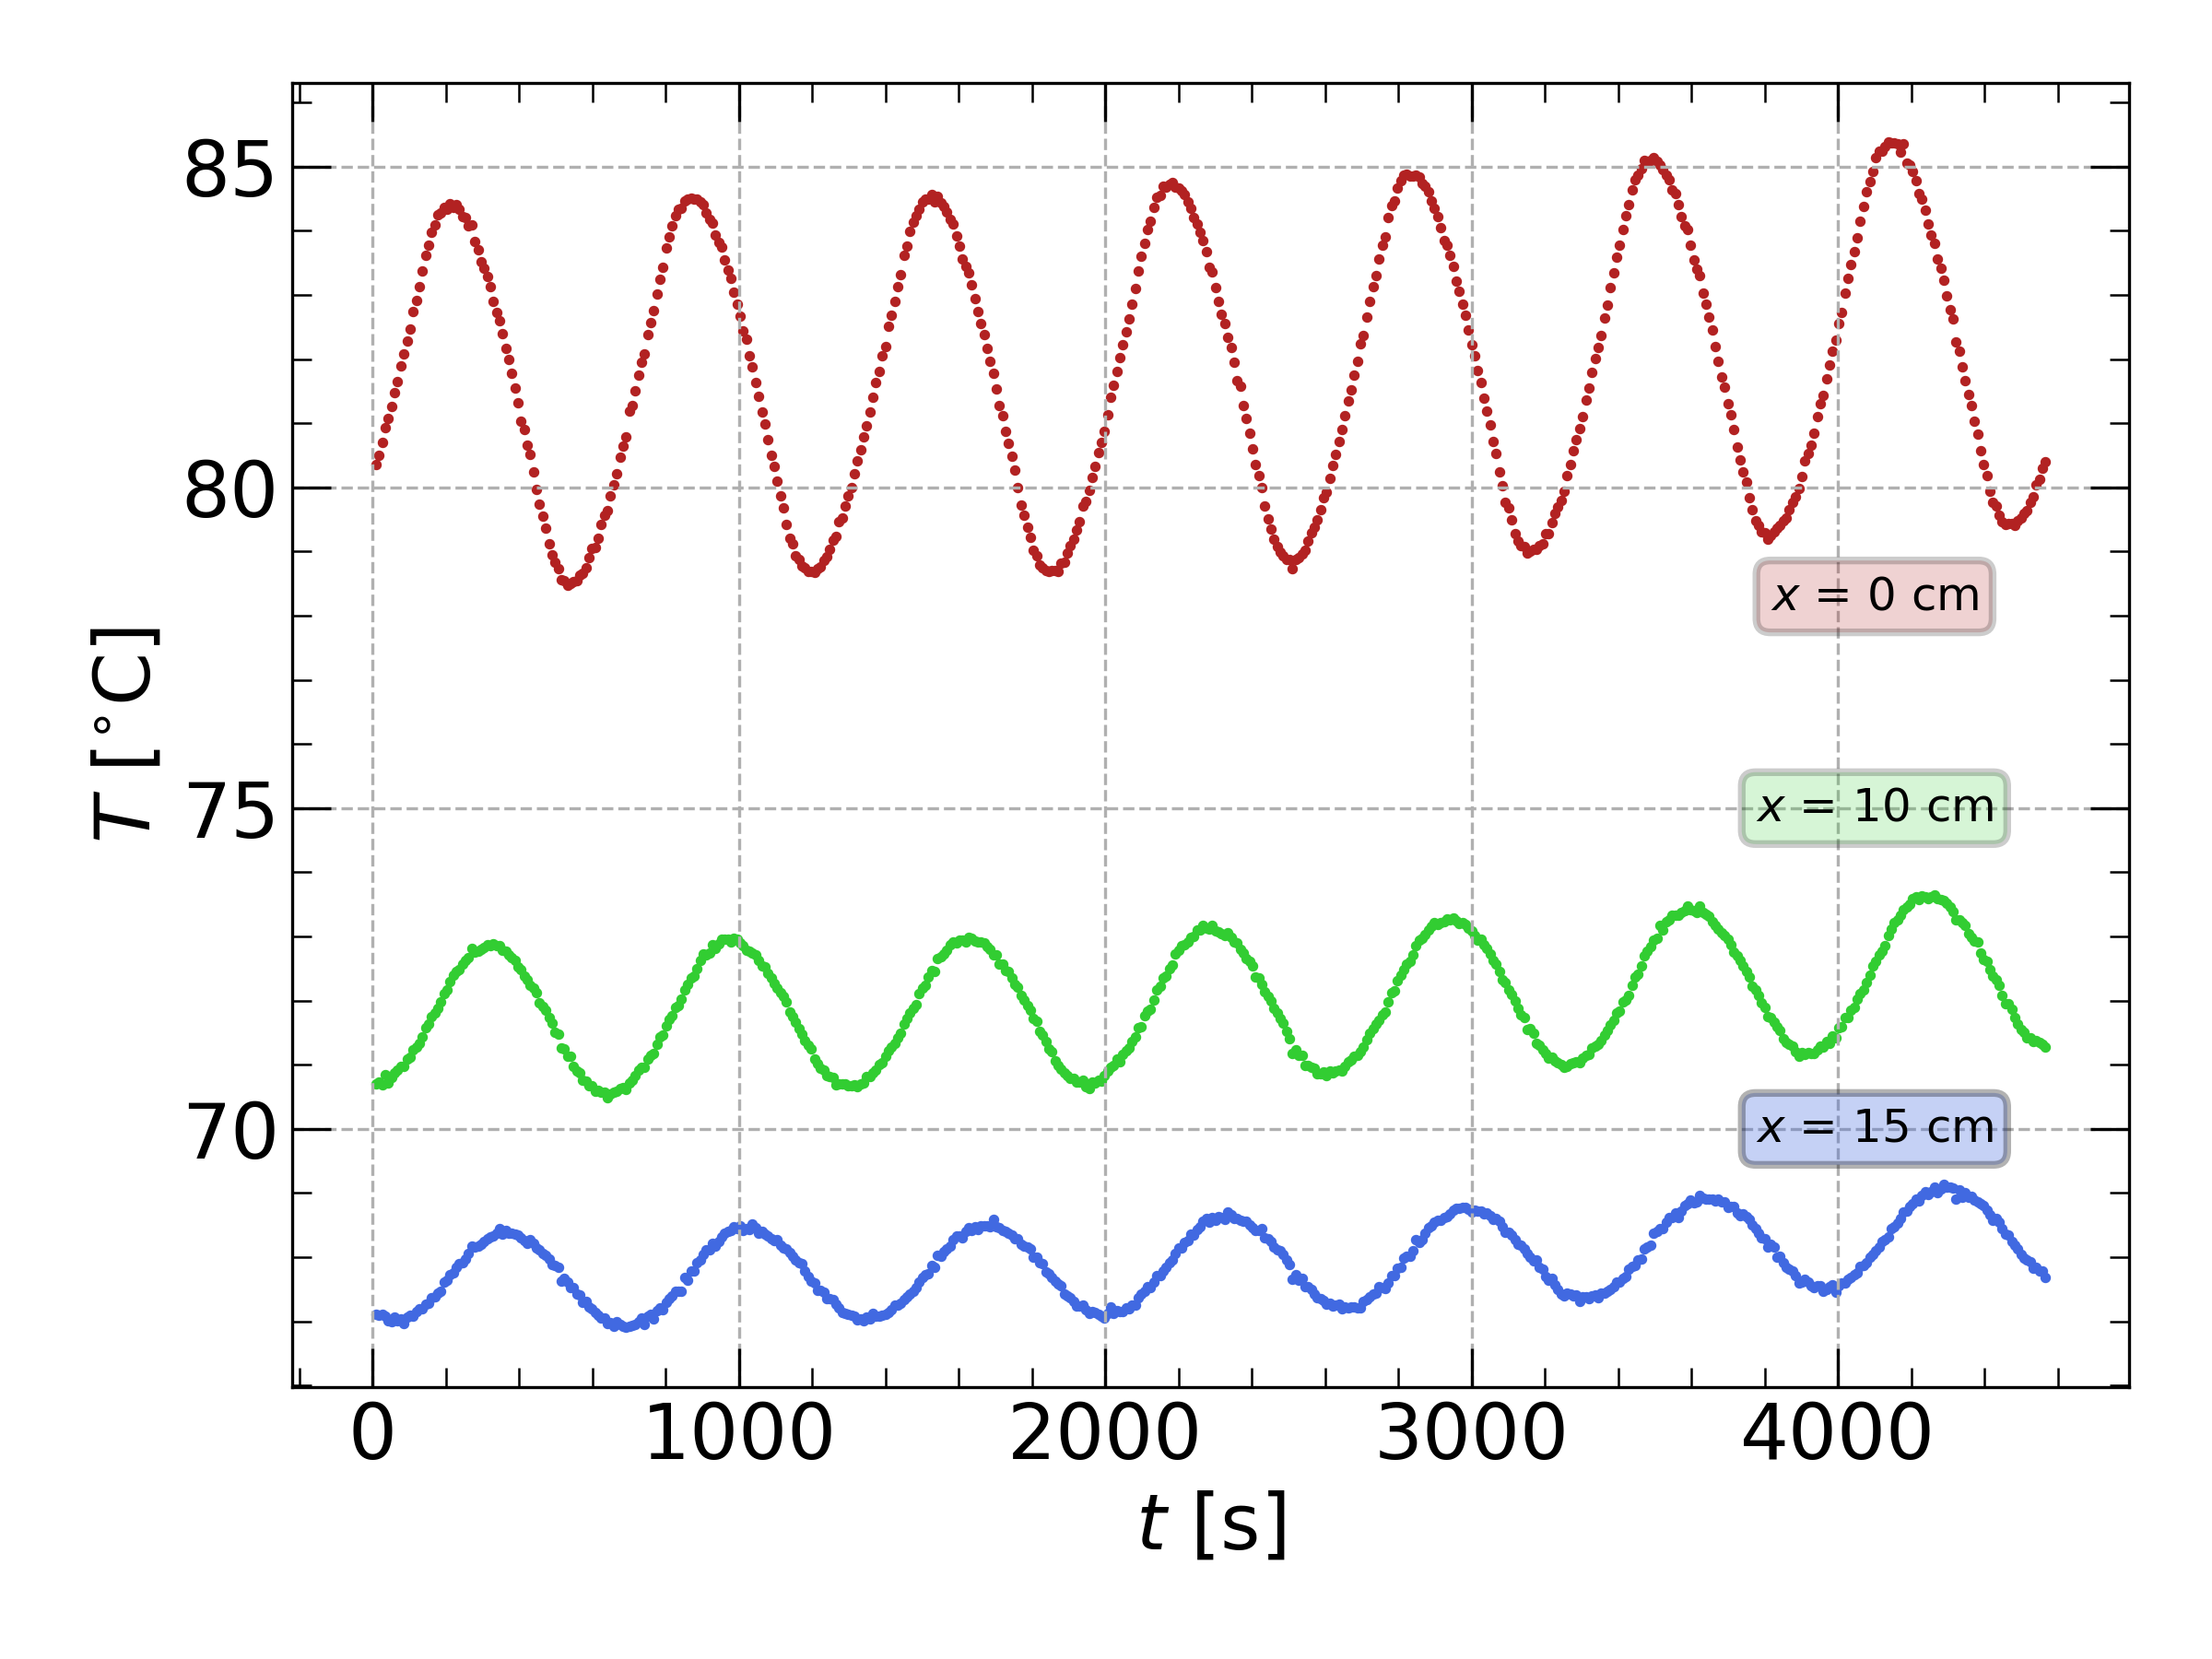
\includegraphics[width= 1\linewidth]{../../graphs/practica_Ia/plots/gran.png}
  \captionof{figure}{T vs t per cada posició. Gran}
  \label{fig:T_vs_t_gran}
\end{Figura}
\begin{Figura}
  \centering
  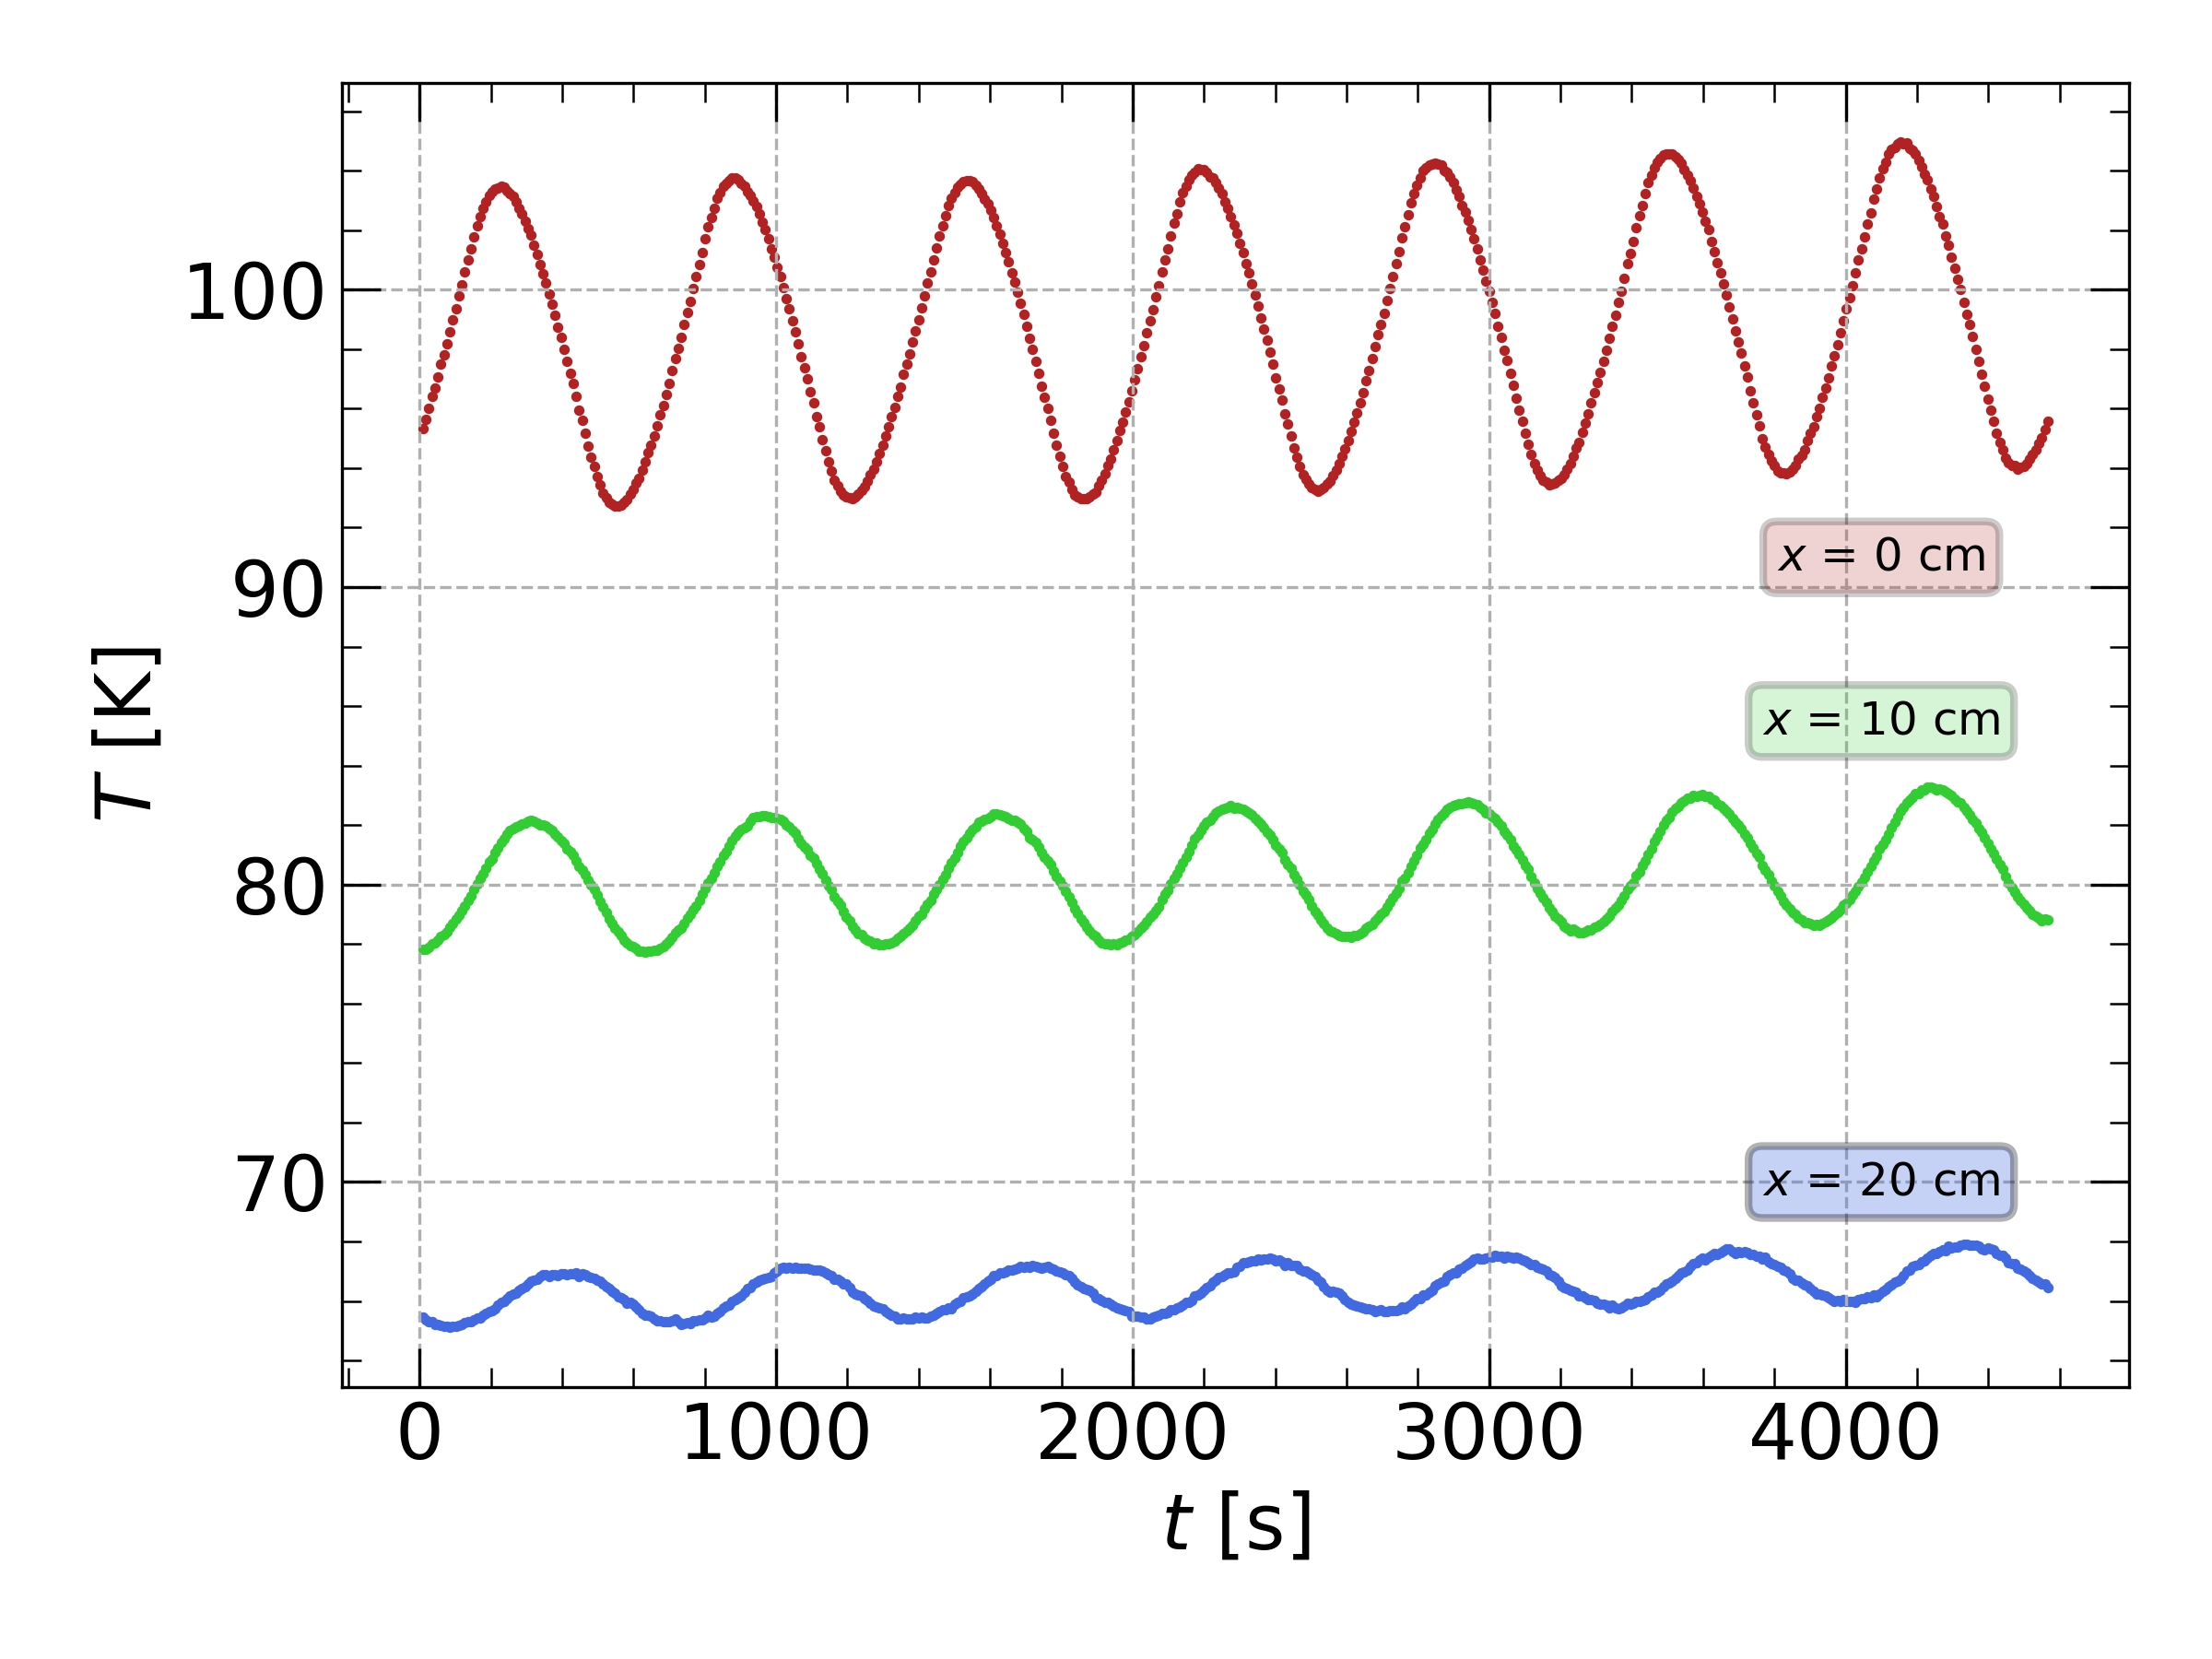
\includegraphics[width= 1\linewidth]{../../graphs/practica_Ia/plots/petita.png}
  \captionof{figure}{T vs t per cada posició. Petita}
  \label{fig:T_vs_t_petita}
\end{Figura}
Notem com l'evolució temporal mesurada de la temperatura és coherent amb la solució de l'equació diferencial vista a l'Equació \eqref{sol_permanent}. (El terme que corresón a la solució de l'estat estacionari no s'aprecia per bla bla bla) El segón terme de la solució correspón a una funció periòdica en el temps que decau amb la distància i presenta un desfasament, també depenent de la distància. Tant a la Figura \ref{fig:T_vs_t_gran} com a la Figura \ref{fig:T_vs_t_petita} es veu que la temperatura és funció periòdica en el temps (ona tèrmica) i que, quant més lluny del punt de referència ens trobem, més petita és l'amplitud de d'aquesta ona. Tot i ser complicat a simple vista veure-ho, existeix un desfasament entre les oscil·lacions de la mateixa barra a diferents distàncies. Per a observar millor aquest desfasament podem preparar les dades d'una forma més convenient.\\\\
Com a pas previ a observar el desfasament, calculem la temperatura mitjana a cada punt de cada barra. Com a simplificació, calculem aquesta mitjana temporal fent una mitjana aritmètica de les dades obtingudes al laboratori. Els valors d'aquestes mitjanes venen recollits a la Taula \ref{Tau:mitjanes}
\begin{Figura}
  \centering
  \captionof{table}{\footnotesize{Temperatura mitjana}}
  \begin{tabular}{c|c|c}
    a & a & a \\
    b & b & b 
  \end{tabular}
  \label{Tau:mitjanes}
\end{Figura}
Observem com la temperatura mitjana decau amb la distància respecte a l'origen de referència. Clarament són pocs punts experimentals com per a traçar una corba de tendència. Tot i això, qualitativament els valors obtinguts s'apropen al que prediu la teoria. En cas de repetir l'experiment amb més termoparells repartits al llarg de cadascuna de les barres observariem un comportament de la mitjana temporal de la temperatura com el de l'Equació \eqref{prom_temp}. Si apliquem el mateix mètode que a l'estat estacionari per a obtenir el valor de $p$ obtenim els valors que s'observen a la Taula \ref{tau:pendent_mitjana}. A partir d'aquestes dades realitzem una regressió i observem, Figura \ref{fig:lin_reg} com s'apropen molt a un comportament lineal.
\begin{Figura}
  \centering
  \captionof{table}{\footnotesize{Pendent del logaritme de les mitjanes}}
  \begin{tabular}{c|c|c}
    a & a & a \\
    b & b & b 
  \end{tabular}
  \label{Tau:pendent_mitjana}
\end{Figura}
\begin{Figura}
  \centering
  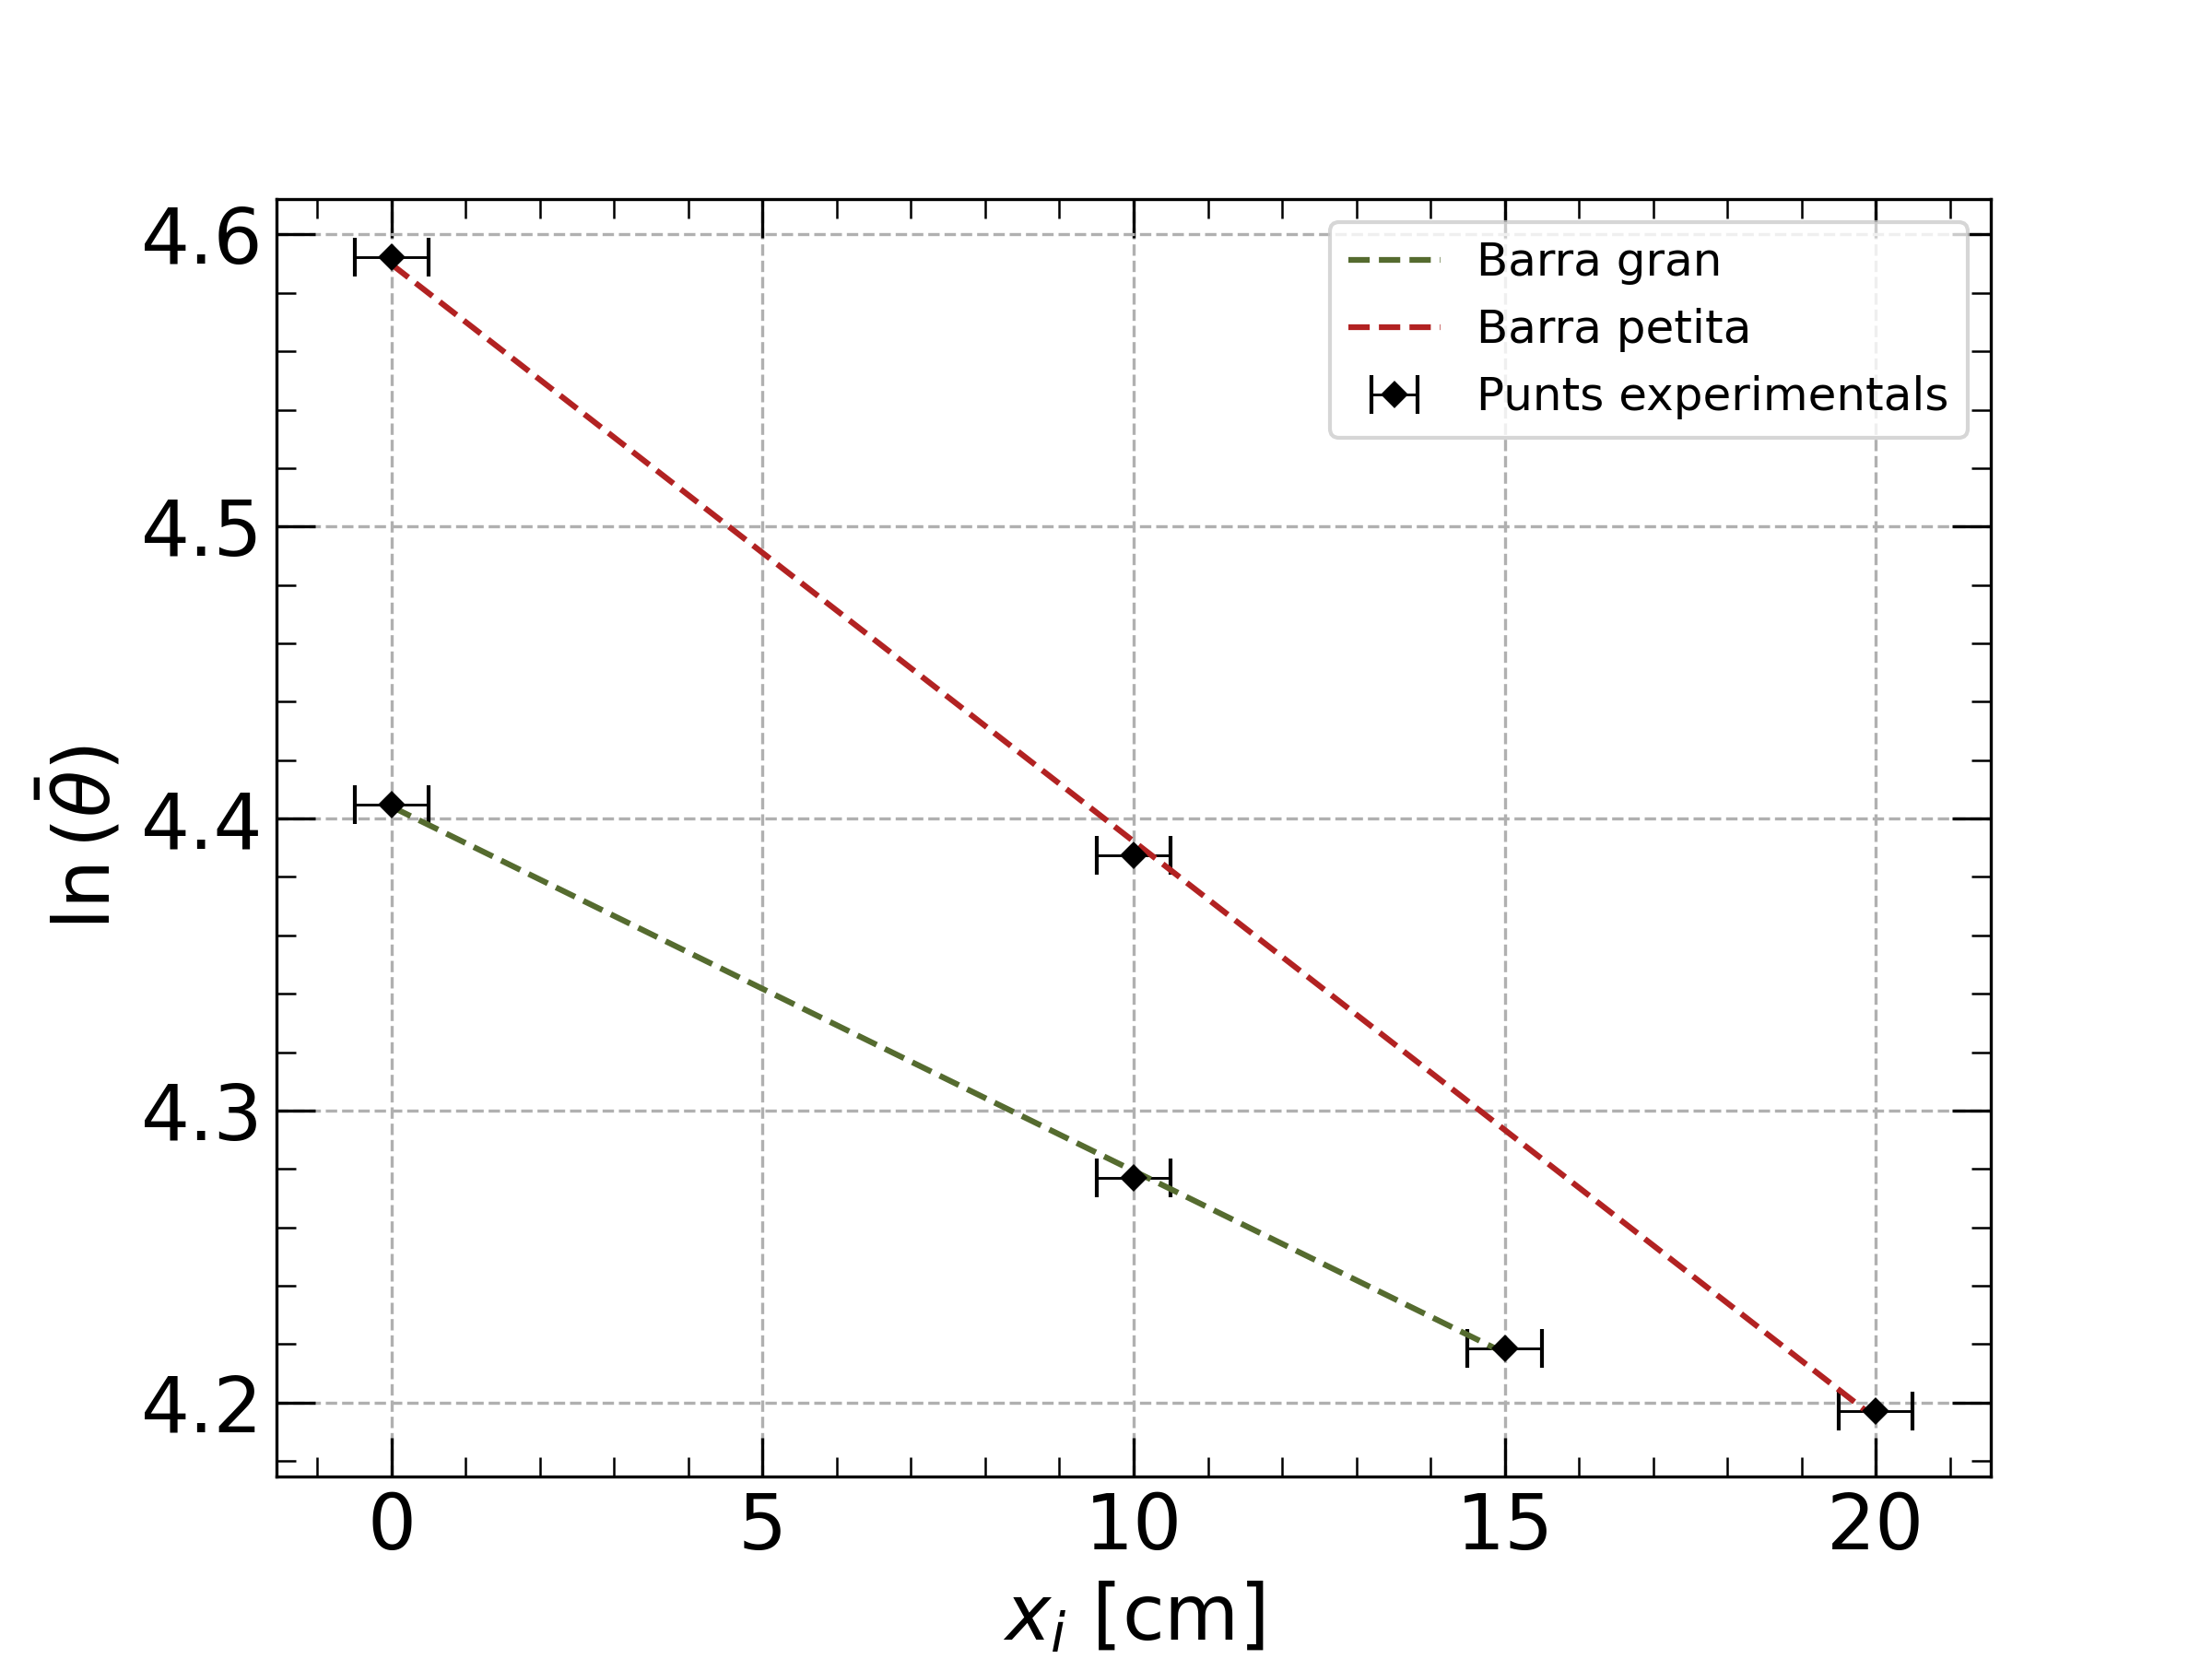
\includegraphics[width=1\linewidth]{../../graphs/practica_Ia/plots/linear_reg.png}
  \captionof{figure}{\footnotesize{regressions lineals de les temperatures mitjanes}}
  \label{fig:lin_reg}
\end{Figura}
Un cop calculades les mitjanes per a cada punt, podem normalitzar les dades experimentals dividint per la seva temperatura mitjana corresponent. Aplicant aquest mètode i, per a obtenir més detall, escollint com a molt els dos primers periodes d'oscil·lació obtenim la Figura \ref{fig:T_vs_t_gran_norm} per a la barra gran i la Figura \ref{fig:T_vs_t_petita_norm} per a la barra petita.
\begin{Figura}
  \centering
  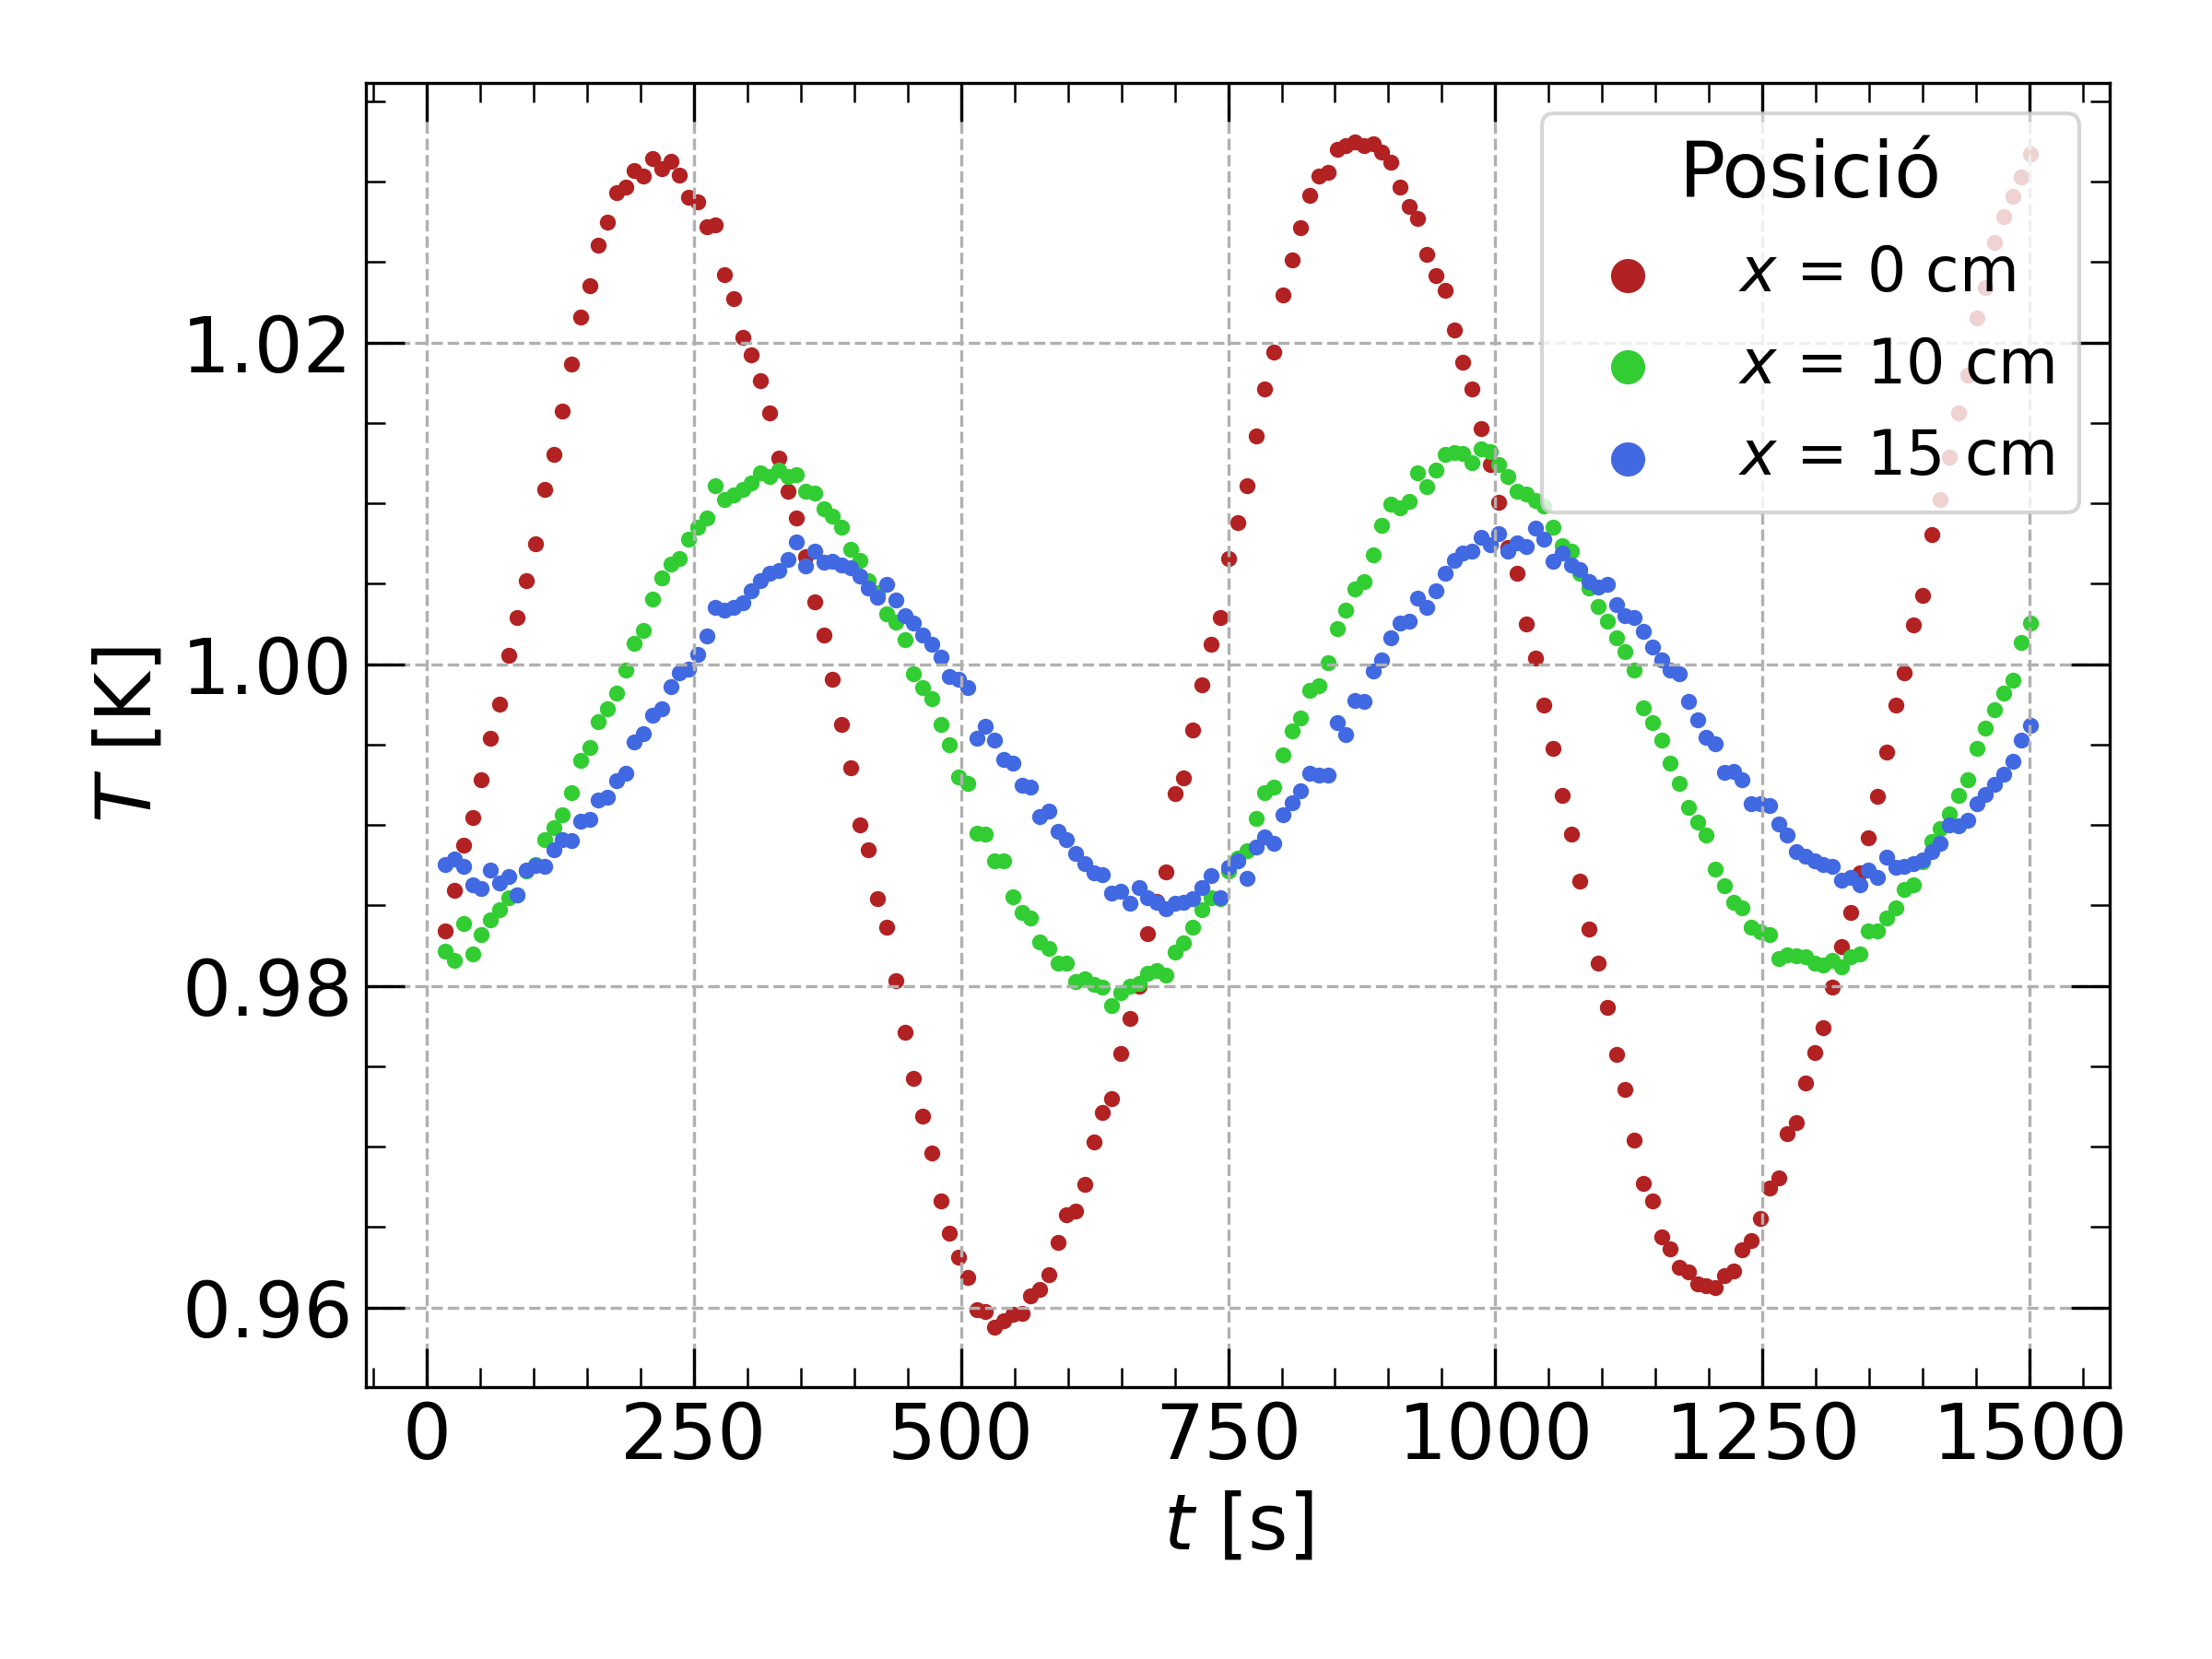
\includegraphics[width=1\linewidth]{../../graphs/practica_Ia/plots/gran_norm.png}
  \captionof{figure}{\footnotesize{Corbes normalitzades per la gran}}
  \label{fig:T_vs_t_gran_norm}
\end{Figura}
\begin{Figura}
  \centering
  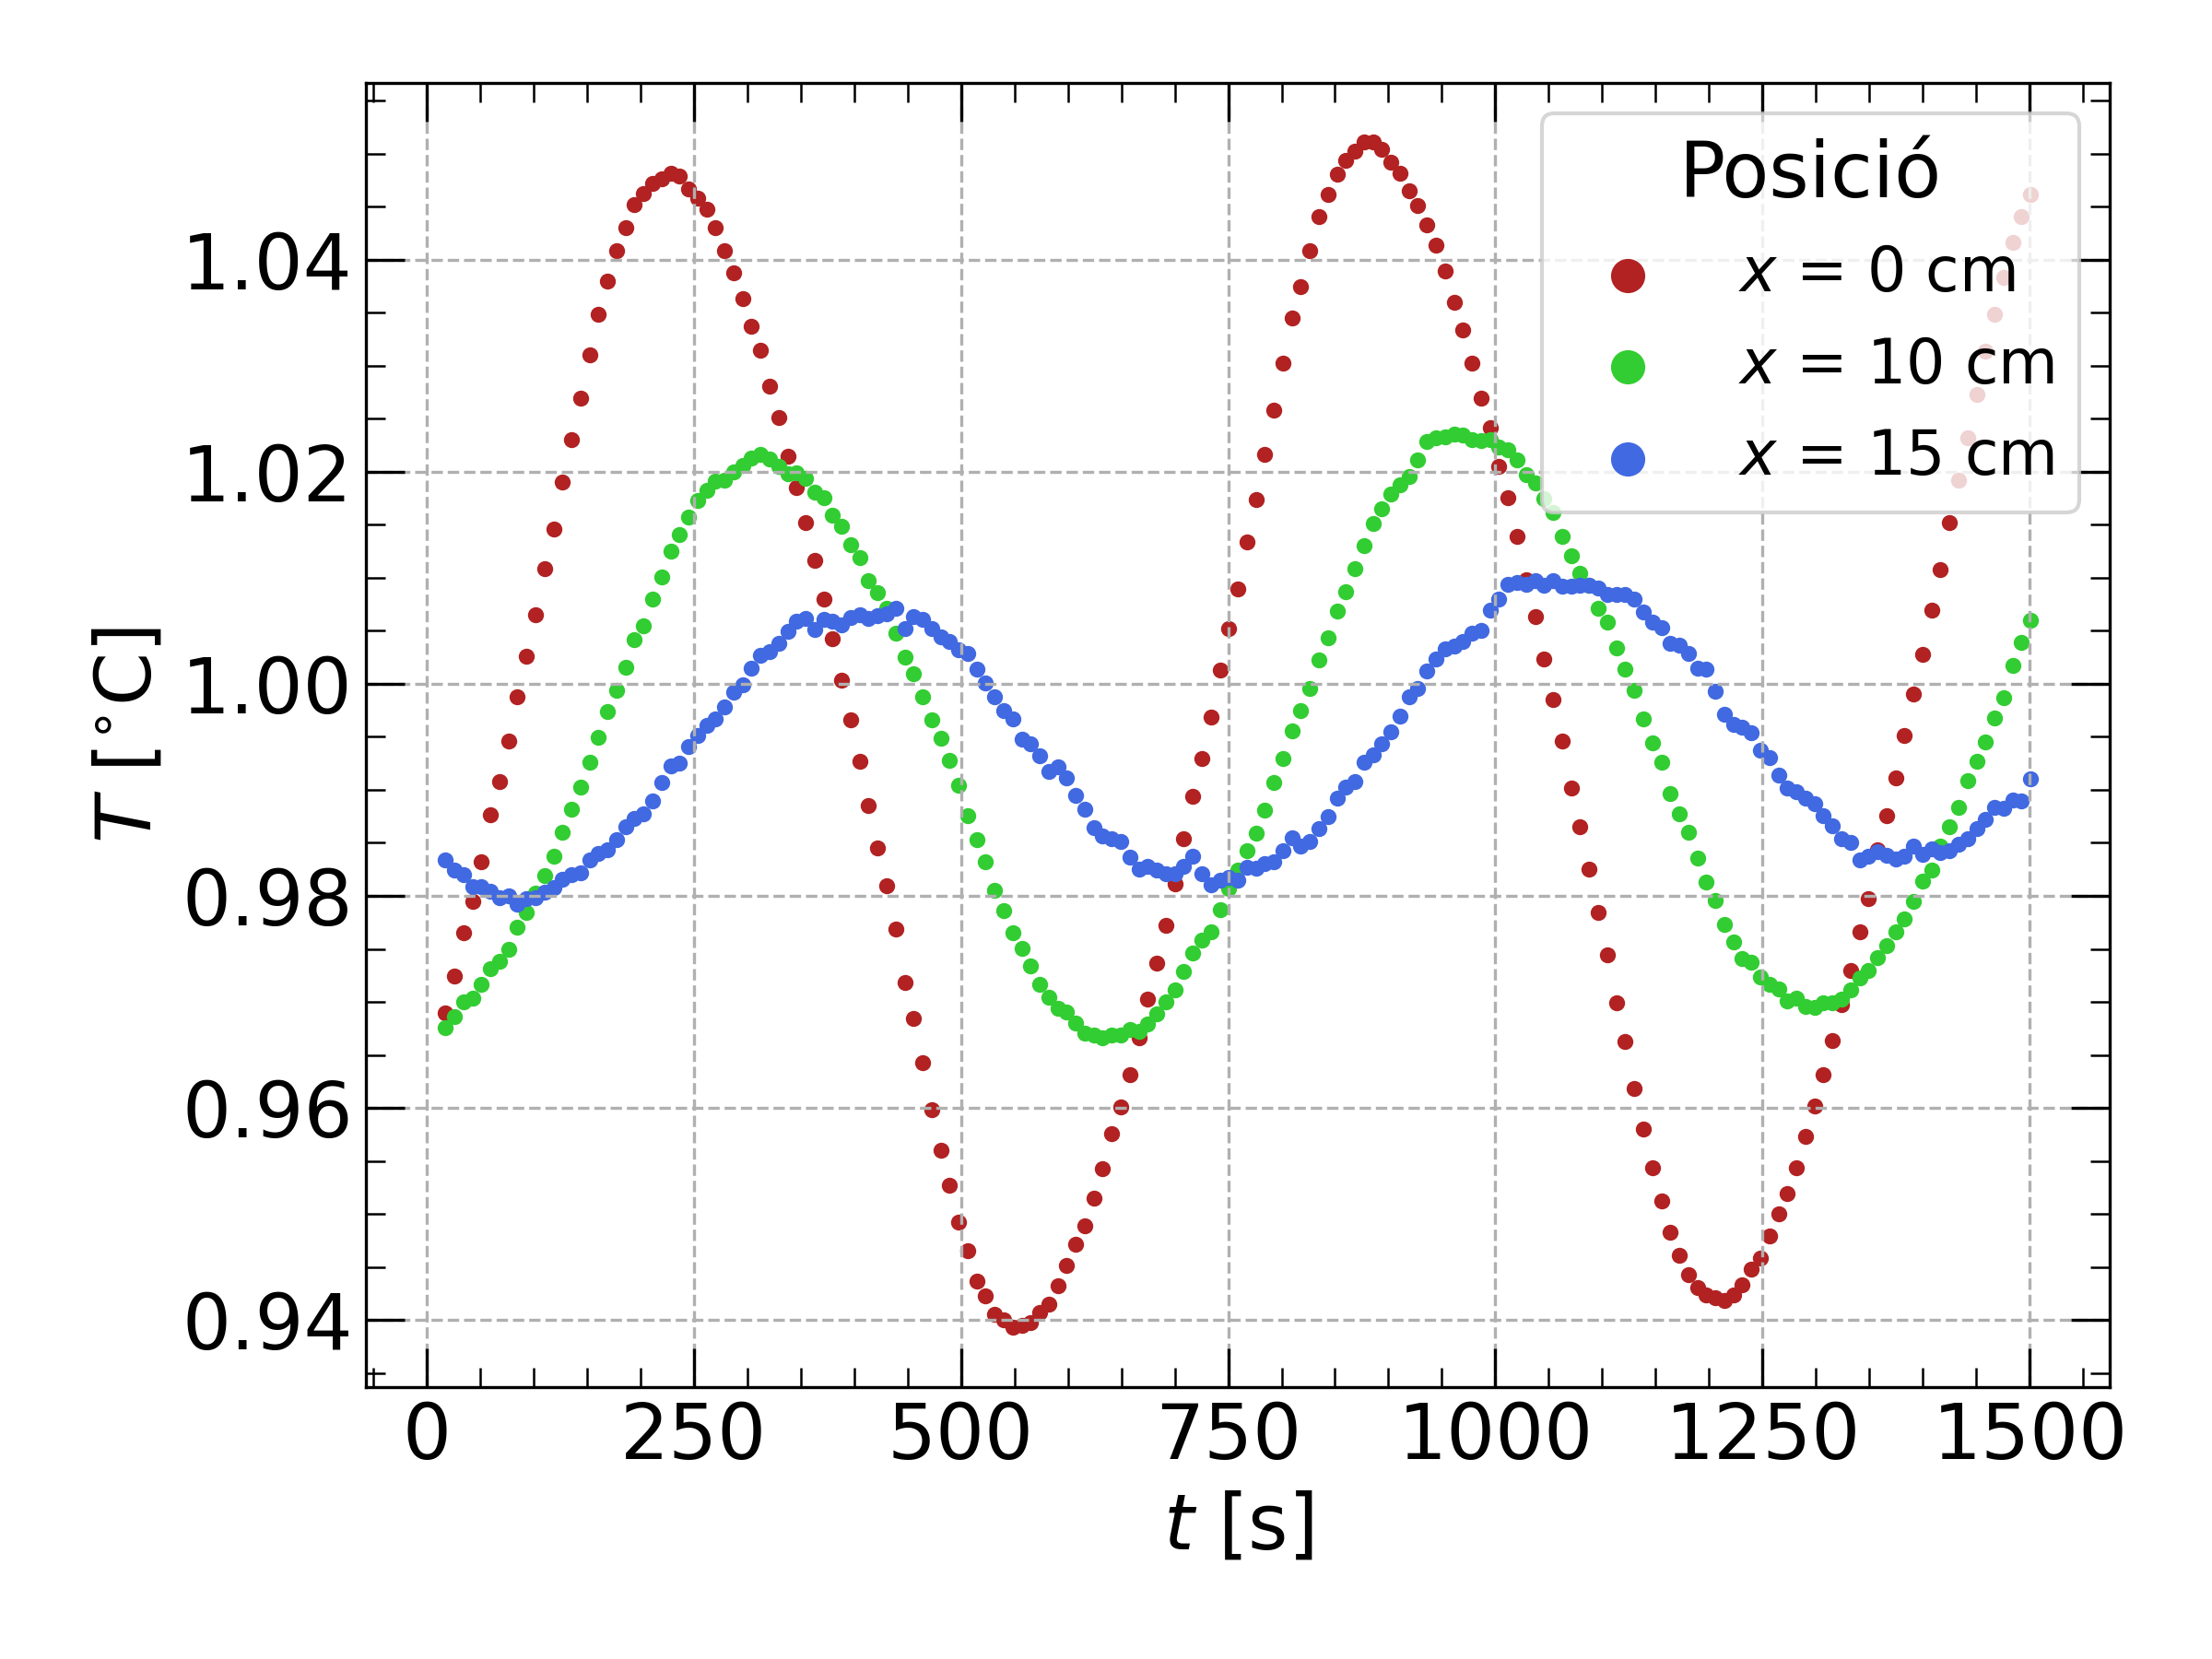
\includegraphics[width=1\linewidth]{../../graphs/practica_Ia/plots/petit_norm.png}
  \captionof{figure}{\footnotesize{Corbes normalitzades per la petita}}
  \label{fig:T_vs_t_petita_norm}
\end{Figura}
Es pot obeservar com existeix desfasament entre dos punts diferents a cada barra, la ona tèrmica avança a mesura que augmenta la distància.\\\\
Per a determinar l'amplitud de la ona a cada punt per a cada barra escollim un punt màxim i un mínim consecutius i calculem la meitat de la diferència. Amb aquestes dades realitzem una mitjana i obtenim les amplituds que s'observen a la Taula \ref{tau:amplituds_mitjanes}.
\begin{Figura}
  \centering
  \captionof{table}{\footnotesize{amplituds mitjanes de la ona a cada punt de l'espai per a cada barra}}
  \begin{tabular}{c|c|c}
    a & a & a \\
    b & b & b 
  \end{tabular}
  \label{tau:amplituds_mitjanes}
\end{Figura} 
Es pot observar com segueixen un comportament exponencial, similar al que hem vist a la Taula \ref{Tau:mitjanes}. Apliquem novament el mateix mètode amb les amplituds que amb les temperatures mitjanes i obtenim les regressions de la Figura \ref{fig:reg_lin_amplituds} i els valors dels pendents de la Taula \ref{tau:pendent_amplituds}.

\begin{Figura}
  \centering
  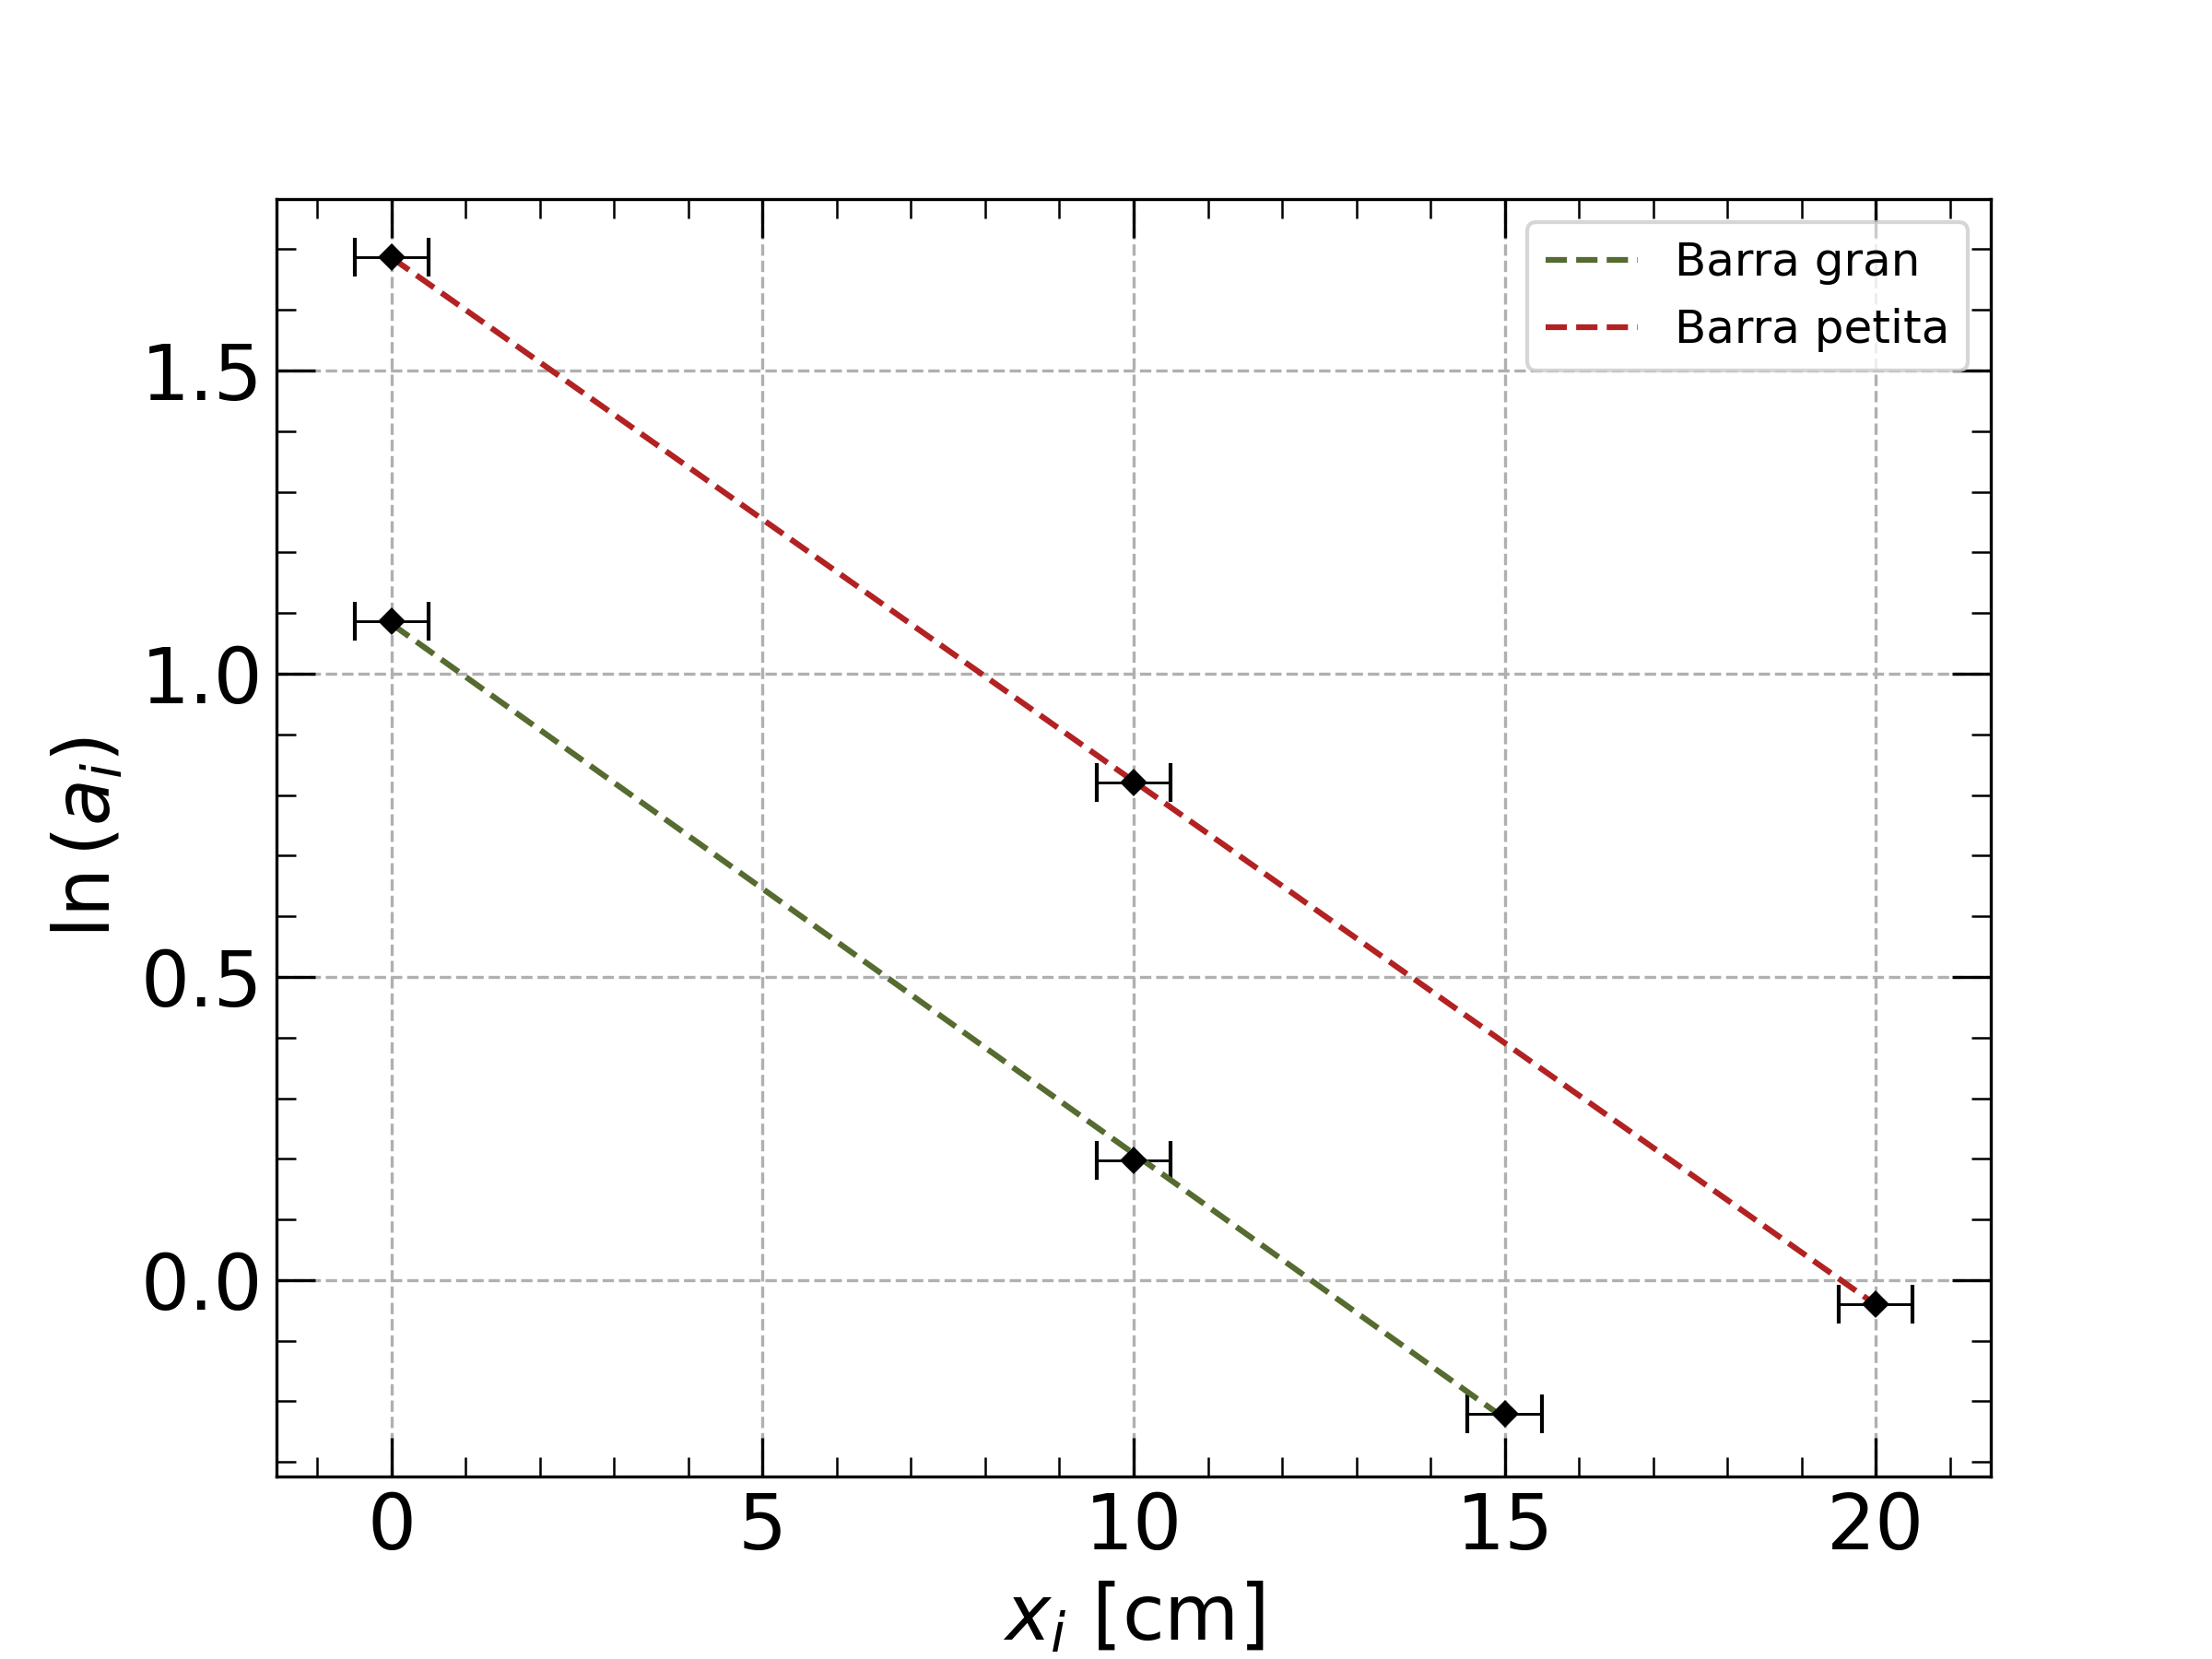
\includegraphics[width=1\linewidth]{../../graphs/practica_Ia/plots/reg_ampli.png}
  \captionof{figure}{\footnotesize{regressions de les amlpituds}}
  \label{fig:reg_lin_amplituds}
\end{Figura}
\begin{Figura}
  \centering
  \captionof{table}{\footnotesize{amplituds mitjanes de la ona a cada punt de l'espai per a cada barra}}
  \begin{tabular}{c|c|c}
    a & a & a \\
    b & b & b 
  \end{tabular}
  \label{tau:pendent_amplituds}
\end{Figura} 
\section{Conclusions}
\end{multicols}
\end{document}
